\documentclass[titlepage, a4paper]{article}
\usepackage[swedish]{babel}
\usepackage[utf8]{inputenc}
\usepackage{color}
\usepackage{graphicx}
\usepackage{etoolbox}
\usepackage{stringenc}
\usepackage{pdfescape}

% Sidformat
\usepackage{a4wide}

% Fixa Appendix-titlar
\usepackage[titletoc,title]{appendix}

% Bättre tabeller
\usepackage{tabularx}

% Bättre bildtexter
\usepackage[margin=10pt,font=small,labelfont=bf,labelsep=endash]{caption}

% Enkelt kommando som låter mig attgöra-markera text
\newcommand{\todo}[1] {\textbf{\textcolor{red}{#1}}}

% Nytt \paragraph låter oss ha onumrerade bitar
\makeatletter
\renewcommand\paragraph{\@startsection{paragraph}{4}{\z@}%
{-3.25ex\@plus -1ex \@minus -.2ex}%
{1.5ex \@plus .2ex}%
{\normalfont\normalsize\bfseries}}
\makeatother

%\providecommand{\LIPSlogga}{../mall/logga1.png}
\providecommand{\LIPSdatum}{\today}

%% Headers och Footers
\usepackage{fancyhdr}
\pagestyle{fancy}
%\lhead{\includegraphics[scale=0.4]{\LIPSlogga}}
\rhead{\ifdef{\LIPSutfardare}{Utfärdat av \LIPSutfardare \\\LIPSdatum}\LIPSdatum}
\lfoot{\LIPSkursnamn \\ \LIPSdokumenttyp}
\cfoot{\thepage}
\rfoot{\LIPSprojektgrupp \\ \LIPSprojektnamn}

%% Titelsida
\newcommand{\LIPSTitelsida}{%
{\ }\vspace{45mm}
\begin{center}
  \textbf{\Huge \LIPSdokument}
\end{center}
\begin{center}
  {\Large Redaktör: \LIPSredaktor}
\end{center}
\begin{center}
  {\Large \textbf{Version \LIPSversion}}
\end{center}
\vfill
\begin{center}
  {\large Status}\\[1.5ex]
  \begin{tabular}{|*{3}{p{40mm}|}}
    \hline
    Granskad & \LIPSgranskare & \LIPSgranskatdatum \\
    \hline
    Godkänd & \LIPSgodkannare & \LIPSgodkantdatum \\
    \hline
  \end{tabular}
\end{center}
\newpage
}

% Projektidentitet
\newenvironment{LIPSprojektidentitet}{%
{\ }\vspace{45mm}
\begin{center}
  {\Large PROJEKTIDENTITET}\\[0.5ex]
  {\small
  \LIPSartaltermin, \LIPSprojektgrupp\\
  Linköpings Tekniska Högskola, IDA
  }
\end{center}
\begin{center}
  {\normalsize Gruppdeltagare}\\
  \begin{tabular}{|l|l|p{25mm}|l|}
    \hline
    \textbf{Namn} & \textbf{Ansvar} & \textbf{Telefon} & \textbf{E-post} \\
    \hline
}%
{%
    \hline
  \end{tabular}
\end{center}
\begin{center}
  {\small
    \ifdef{\LIPSgruppadress}{\textbf{E-postlista för hela gruppen}: \LIPSgruppadress\\}{}
    \ifdef{\LIPSgrupphemsida}{\textbf{Hemsida}: \LIPSgrupphemsida\\[1ex]}{}
    \ifdef{\LIPSkund}{\textbf{Kund}: \LIPSkund\\}{}
    \ifdef{\LIPSkundkontakt}{\textbf{Kontaktperson hos kund}: \LIPSkundkontakt\\}{}
    \ifdef{\LIPSkursansvarig}{\textbf{Kursansvarig}: \LIPSkursansvarig\\}{}
    \ifdef{\LIPShandledare}{\textbf{Handledare}: \LIPShandledare\\}{}
  }
\end{center}
\newpage
}
\newcommand{\LIPSgruppmedlem}[4]{\hline {#1} & {#2} & {#3} & {#4} \\}

%% Dokumenthistorik
\newenvironment{LIPSdokumenthistorik}{%
\begin{center}
  Dokumenthistorik\\[1ex]
  %\begin{small}
    \begin{tabular}{|l|l|p{60mm}|l|l|}
      \hline
      \textbf{Version} & \textbf{Datum} & \textbf{Utförda förändringar} & \textbf{Utförda av} & \textbf{Granskad} \\
      }%
    {%
			\hline
    \end{tabular}
  %\end{small}
\end{center}
}

\newcommand{\LIPSversionsinfo}[5]{\hline {#1} & {#2} & {#3} & {#4} & {#5} \\}

% Kravlistor
\newenvironment{LIPSkravlista}{
	\center
		\tabularx{\textwidth}{| p{1.2cm} | p{1.9cm} | X | c |}
			\hline
			\textbf{Krav} & \textbf{Förändring} & \textbf{Beskrivning} & \textbf{Prioritet} \\\hline
}
{
		\endtabularx
	\endcenter
}

\newcounter{LIPSkravnummer}
\addtocounter{LIPSkravnummer}{1}
\newcommand{\LIPSkrav}[4][Krav \arabic{LIPSkravnummer}]{{#1} & {#2} & {#3} & {#4} \stepcounter{LIPSkravnummer}\\\hline}


% Leveranskravlistor
\newenvironment{LIPSleveranskravlista}{
	\center
		\tabularx{\textwidth}{| p{1.2cm} | p{1.9cm} | X | X |}
			\hline
			\textbf{Krav} & \textbf{Förändring} & \textbf{Beskrivning} & \textbf{Deadline}\\\hline
}
{
		\endtabularx
	\endcenter
}

\newcounter{LIPSleveranskravnummer}
\addtocounter{LIPSleveranskravnummer}{1}
\newcommand{\LIPSleveranskrav}[4][Krav \arabic{LIPSkravnummer}]{{#1} & {#2} & {#3} & {#4} \stepcounter{LIPSkravnummer}\\\hline}


% Milstolps-lista
\newenvironment{LIPSmilstolpar}{
	\center
		\tabularx{\textwidth}{| p{1.2cm} | X | l |}
			\hline
			\textbf{Nr} & \textbf{Beskrivning} & \textbf{Datum} \\\hline
}
{
		\endtabularx
	\endcenter
}

\newcounter{LIPSstolpnummer}
\addtocounter{LIPSstolpnummer}{1}
%\newcommand{\LIPSmilstolpe}[3][Krav \arabic{LIPSstolpnummer}]{{#1} & {#2} & {#3} \stepcounter{LIPSstolpnummer}\\\hline}
\newcommand{\LIPSmilstolpe}[3]{{#1} & {#2} & {#3} \\\hline}

% Aktivitets-lista
\newenvironment{LIPSaktivitetslista}{
	\center
		\tabularx{\textwidth}{| p{0.3cm} | X | c | c | c |}
			\hline
			\textbf{Nr} & \textbf{Beskrivning} & \textbf{Beroende av} & \textbf{Timmar} & \textbf{datum} \\\hline
}
{
		\endtabularx
	\endcenter
}

\newcounter{LIPSaktivitetsnummer}
\addtocounter{LIPSaktivitetsnummer}{1}
% \newcommand{\LIPSaktivitet}[4][\arabic{LIPSstolpnummer}]{{#1} & {#2} & {#3} & {#4} \stepcounter{LIPSstolpnummer}\\\hline}
\newcommand{\LIPSaktivitet}[5]{{#1} & {#2} & {#3} & {#4} & {#5}\\\hline}

% Mall för mötesprotokoll
\newenvironment{projektmote}[2]{
  {\ }\vspace{5mm}

  \centerline{\textbf{\Huge #1}}
  \vspace{2mm}
  \centerline{\LARGE #2}
  \vspace{10mm}

  \begin{itemize}
}
{
  \end{itemize}
}

\newcounter{paragrafnummer}
\addtocounter{paragrafnummer}{1}
\newcommand{\paragraf}[1]{\item{\textsection \arabic{paragrafnummer}. {#1}}\addtocounter{paragrafnummer}{1}}

% Mall för Statusrapport
\newenvironment{statusrapport}{
  \center
    \tabularx{\textwidth}{| p{0.4cm} | X | X | p{14.5mm} | p{13.5mm} | p{16.5mm} | p{16.5mm} |}
    \hline
    \textbf{Nr} & \textbf{Aktivitet} & \textbf{Beroenden} & \textbf{Planerad tid} & \textbf{Nedlagd tid} & \textbf{Planerad klar} & \textbf{Beräknat klart} \\\hline
}
{
    \endtabularx
  \endcenter
}

\newcommand{\aktivitetstatus}[7]{{#1} & {#2} & {#3} & {#4} & {#5} & {#6} & {#7} \\\hline}	% Importera generella layout-strukturer

% Information nödvändig för generella layout-strukturer
\newcommand{\LIPSredaktor}{Johannes Klasson}
\newcommand{\LIPSversion}{P1B}
\newcommand{\LIPSdokument}{High-Level Design Report}
\newcommand{\LIPSdokumenttyp}{High-Level Design Report}
\newcommand{\LIPSgranskatdatum}{2016-02-15}
\newcommand{\LIPSgranskare}{Johannes Klasson}
\newcommand{\LIPSgodkannare}{Martin Nielsen-Lönn}
\newcommand{\LIPSgodkantdatum}{-}
\newcommand{\LIPSkursnamn}{TSEK06}
\newcommand{\LIPSprojektnamn}{16-bit Kogge-Stone Adder}
\newcommand{\LIPSprojektgrupp}{Group 5}
\newcommand{\LIPSartaltermin}{VT, 2016}
\newcommand{\LIPSkund}{ISY}
\newcommand{\LIPSkundkontakt}{Martin Nielsen-Lönn}
\newcommand{\LIPSkursansvarig}{Atila Alvandpour}
\newcommand{\LIPShandledare}{Martin Nielsen-Lönn}

% Dokument-specifika paket
\usepackage{tabularx}
\usepackage{pdfpages}
\usepackage{tikz}
\usepackage{float}
\usetikzlibrary{shapes, arrows}
\usepackage{booktabs} % Horizontal rules in tables
\usepackage[justification=centering]{caption}
\usepackage{adjustbox}
\pagenumbering{roman}


\DeclareGraphicsRule{.0.pdf}{pdf}{*}{}

\begin{document}

\LIPSTitelsida

\begin{LIPSprojektidentitet}
  \LIPSgruppmedlem{Johan Isaksson}{Project Leader}{070-2688785}{johis024@student.liu.se}
  \LIPSgruppmedlem{Johannes Klasson}{Document Manager}{073-8209003}{johkl226@student.liu.se}
  \LIPSgruppmedlem{Jonas Tarasso}{Designer}{070-5738583}{jonta760@student.liu.se}
  \LIPSgruppmedlem{Alexander Yngve}{Designer}{076-2749762}{aleyn573@student.liu.se}	
\end{LIPSprojektidentitet}

\newpage
\tableofcontents	%Innehållsförteckning
%\listoffigures
%\listoftables

\newpage

\begin{LIPSdokumenthistorik}
\LIPSversionsinfo{P1A}{2016-02-15}{First draft}{Johan Isaksson}
\end{LIPSdokumenthistorik}

\newpage
\pagenumbering{arabic}	%Påbörja sidnumrering

% Inledning, översikt osv

\section{Introduction}
This document describes the state of the 16-bit Kogge-Stone adder project in the course TSEK06 after finishing the high level design phase. The system itself is supposed to receive two numbers that should be added together. The result should then both sent out from the system and be compared with a checksum in a BIST (Built-In Self-Test). The meaning of high level is that every basic logic gate is implemented in Verilog-A. The main reason for doing this is to be able to simulate all logic to make sure that everything works as intended. Block level diagrams can be found in section \ref{sec:block_level}, simulation results in section \ref{sec:simulation_results} and a risk analysis in section \ref{sec:risks}. In appendix \ref{app:time_plan} and \ref{app:time_report} a time plan of the next phase and a time report of this phase can be found.


\section{Block Level Description}

\subsection{SPI\_in/PSBR}
The SPI\_in module consists of a lot of registers and some control logic moving data between these registers. Since the PRBS module share some registers with the SPI\_in module, and the PRBS module is relatively small, we included it in the SPI\_in module. \\
The first block in the SPI\_in module is the SPI\_recieve block. It consists of 16 resettable D flip-flops (DFFSR), that is connected one after another. They are clocked on the SPI clock, and on each positive clock pulse, we got a new bit to shift in. After 16 pulses we have 16 bits stored, and a load signal is triggered so that each bit is moved to the correct PRBS-register. \\
The PRBS-registers are register that consists of four DFFSR (one for each addition) and that can be run in two different modes. During the first mode, the normal mode, the registers are triggered with a load signal, and the data to the first DFFSR comes from the SPI\_recieve block. During the second mode, the PRBS mode, the registers and triggered with the system clock, and the data to the first DFFSR is the value of the third and forth DFFSR passed trhough a XOR. The mode is choosen by the SPI\_enable signal.
\subsection{16-bit Kogge-Stone Adder}
The Kogge-Stone adder consists of four simple blocks connected in a complex way, as can be seen in \ref{fig:ks_block}. These four blocks can be seen in figure \ref{fig:red}-\ref{fig:sum}. The red block constitute the initial stage which takes two binary numbers $A$ and $B$ as input. The corresponding truth table is found in table \ref{tab:red} in appendix \ref{app:ks_truth}. The output signals $P$ and $G$ generated from this block are later used by other blocks in the adder. The $G$, also called the Generate signal, trickles down through the hierarchy of yellow, and yellow carry blocks to finally end up in the sum block. The truth table for this block can be found in table \ref{tab:sum}. Truth tables for the yellow and yellow carry blocks are found in table \ref{tab:yellow} and \ref{tab:yellowcarry}.

\begin{figure}[H]
  \centering
  \captionsetup{justification=centering}
  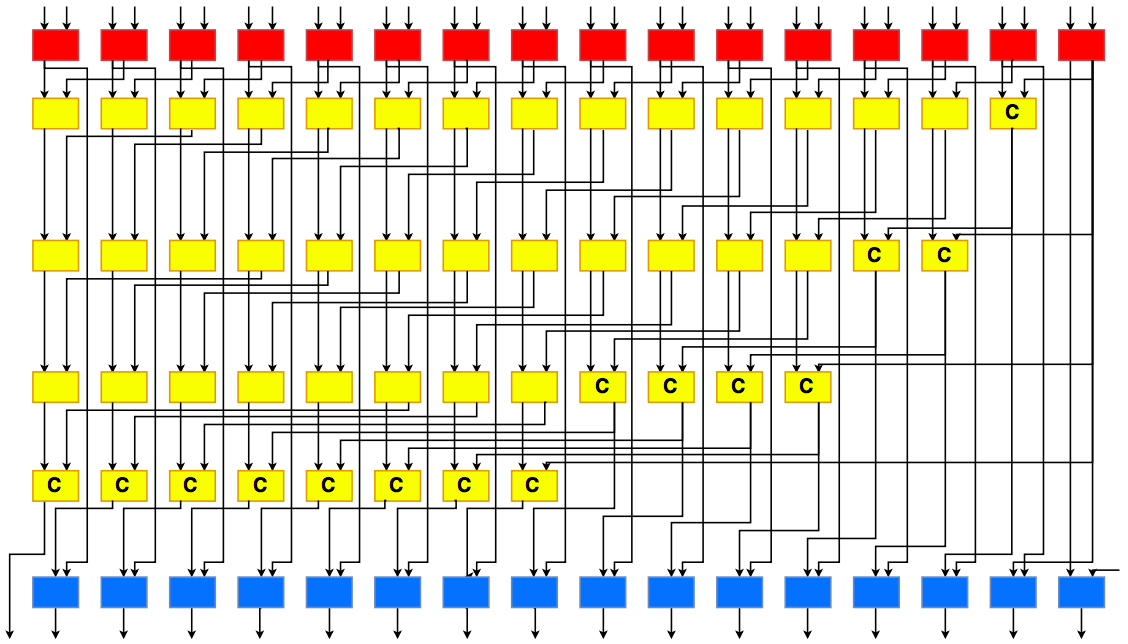
\includegraphics[scale=0.5, angle=90]{../figures/ks_block}
  \caption{Block diagram of the adder.} \label{fig:ks_block}
\end{figure}

\begin{figure}[H]
  \centering
  \captionsetup{justification=centering}
  \adjustbox{trim={.3\width} {0\height} {.3\width} {0\height},clip}
  {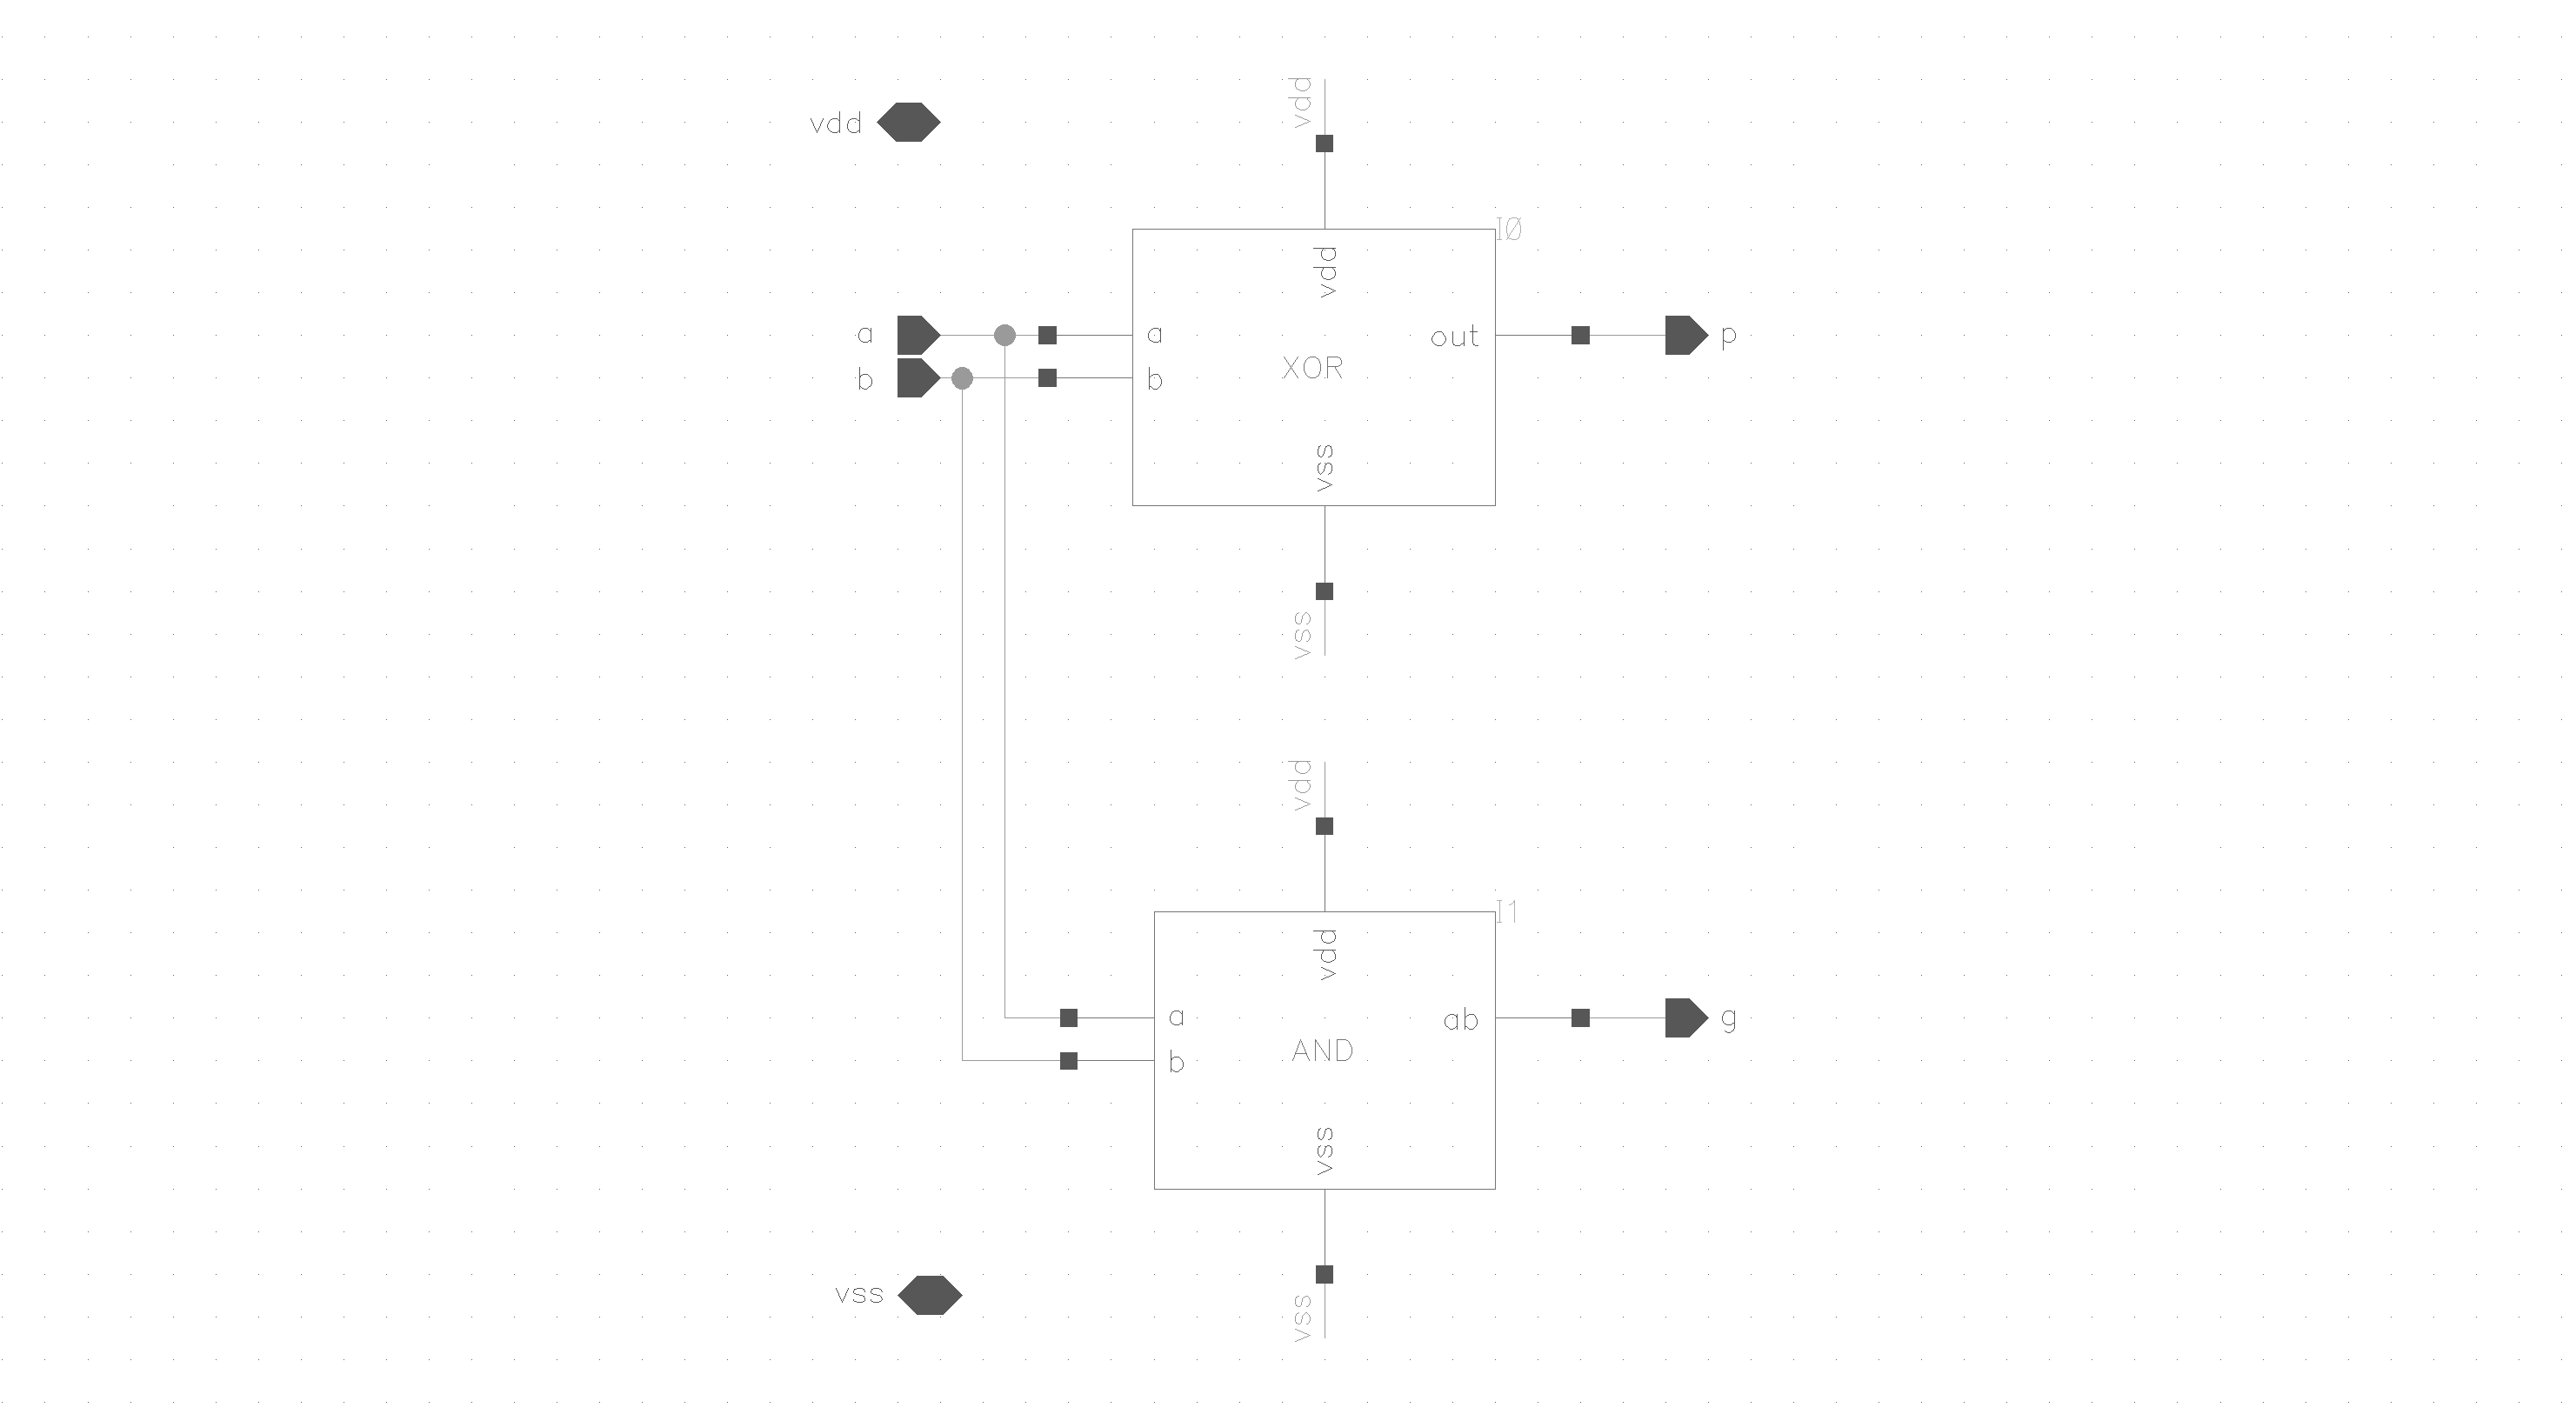
\includegraphics[width=2.0\textwidth]{../figures/red}}
  \caption{Schematic view of the red block.} \label{fig:red}
\end{figure}

\begin{figure}[H]
  \centering
  \captionsetup{justification=centering}
  \adjustbox{trim={.15\width} {0\height} {.12\width} {0\height},clip}
  {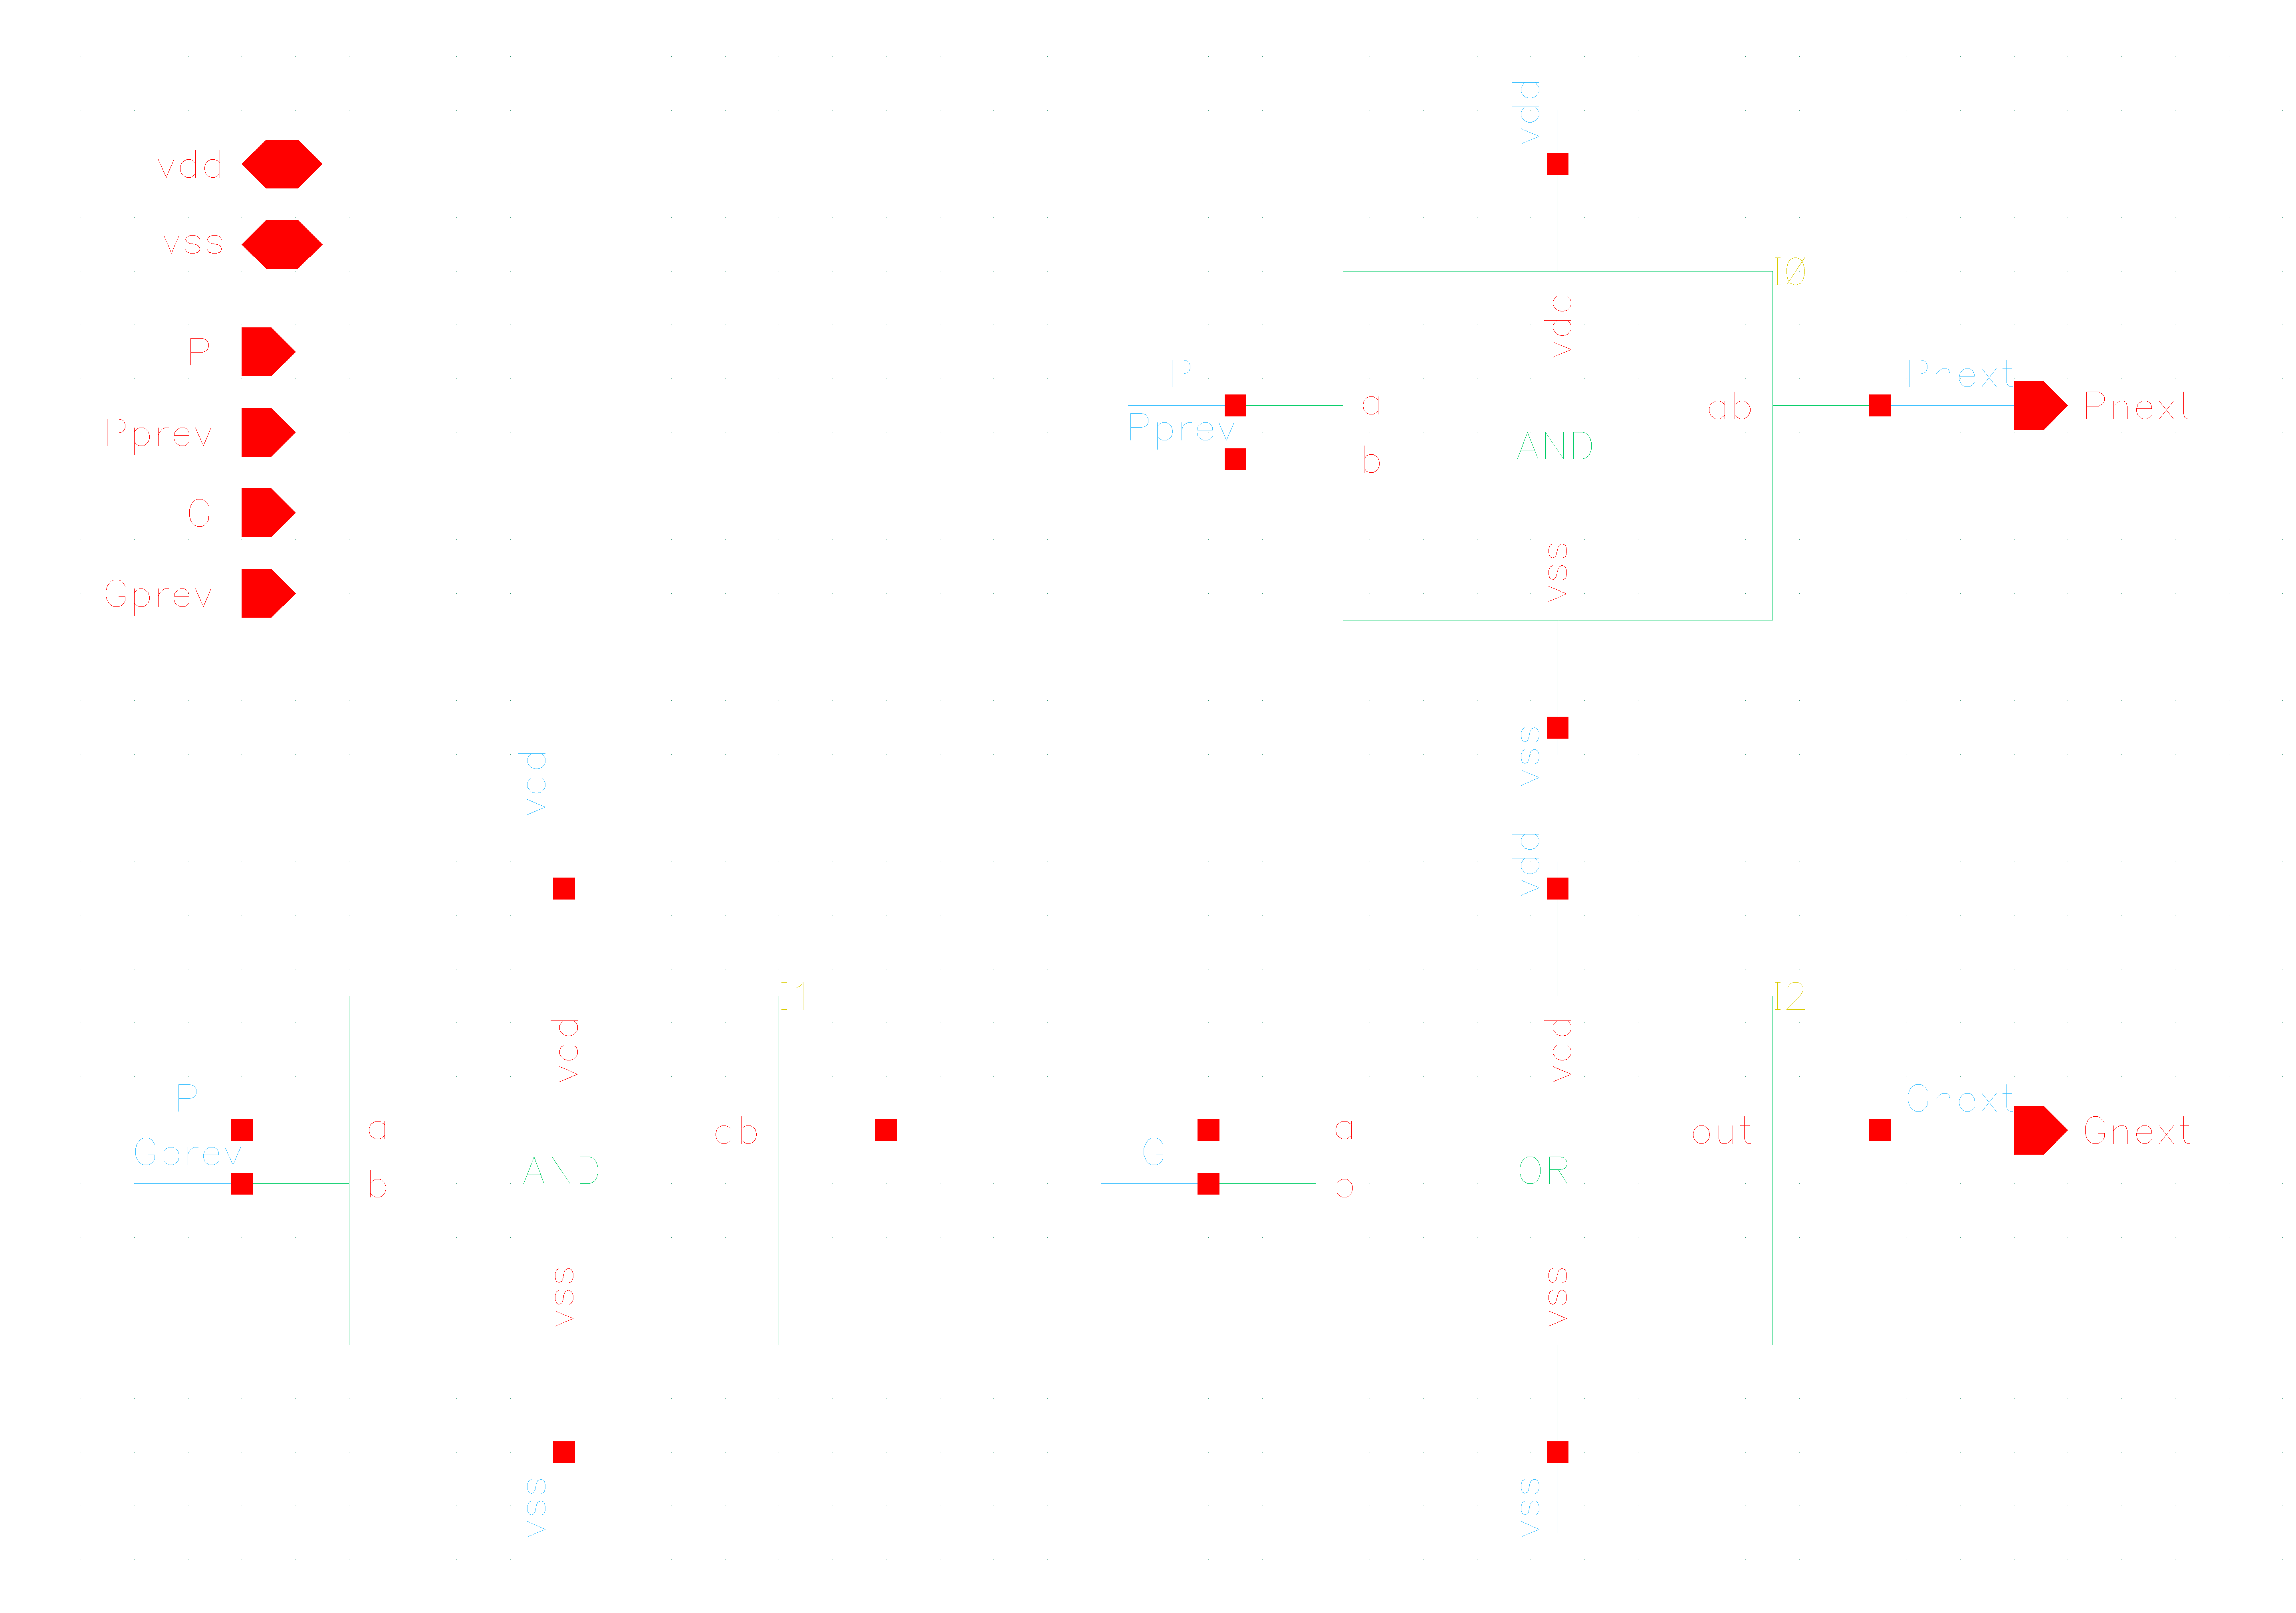
\includegraphics[width=1.3\textwidth]{../figures/yellow}}
  \caption{Schematic view of the yellow block.} \label{fig:yellow}
\end{figure}

\begin{figure}[H]
  \centering
  \captionsetup{justification=centering}
  \adjustbox{trim={.1\width} {0\height} {.1\width} {.4\height},clip}
  {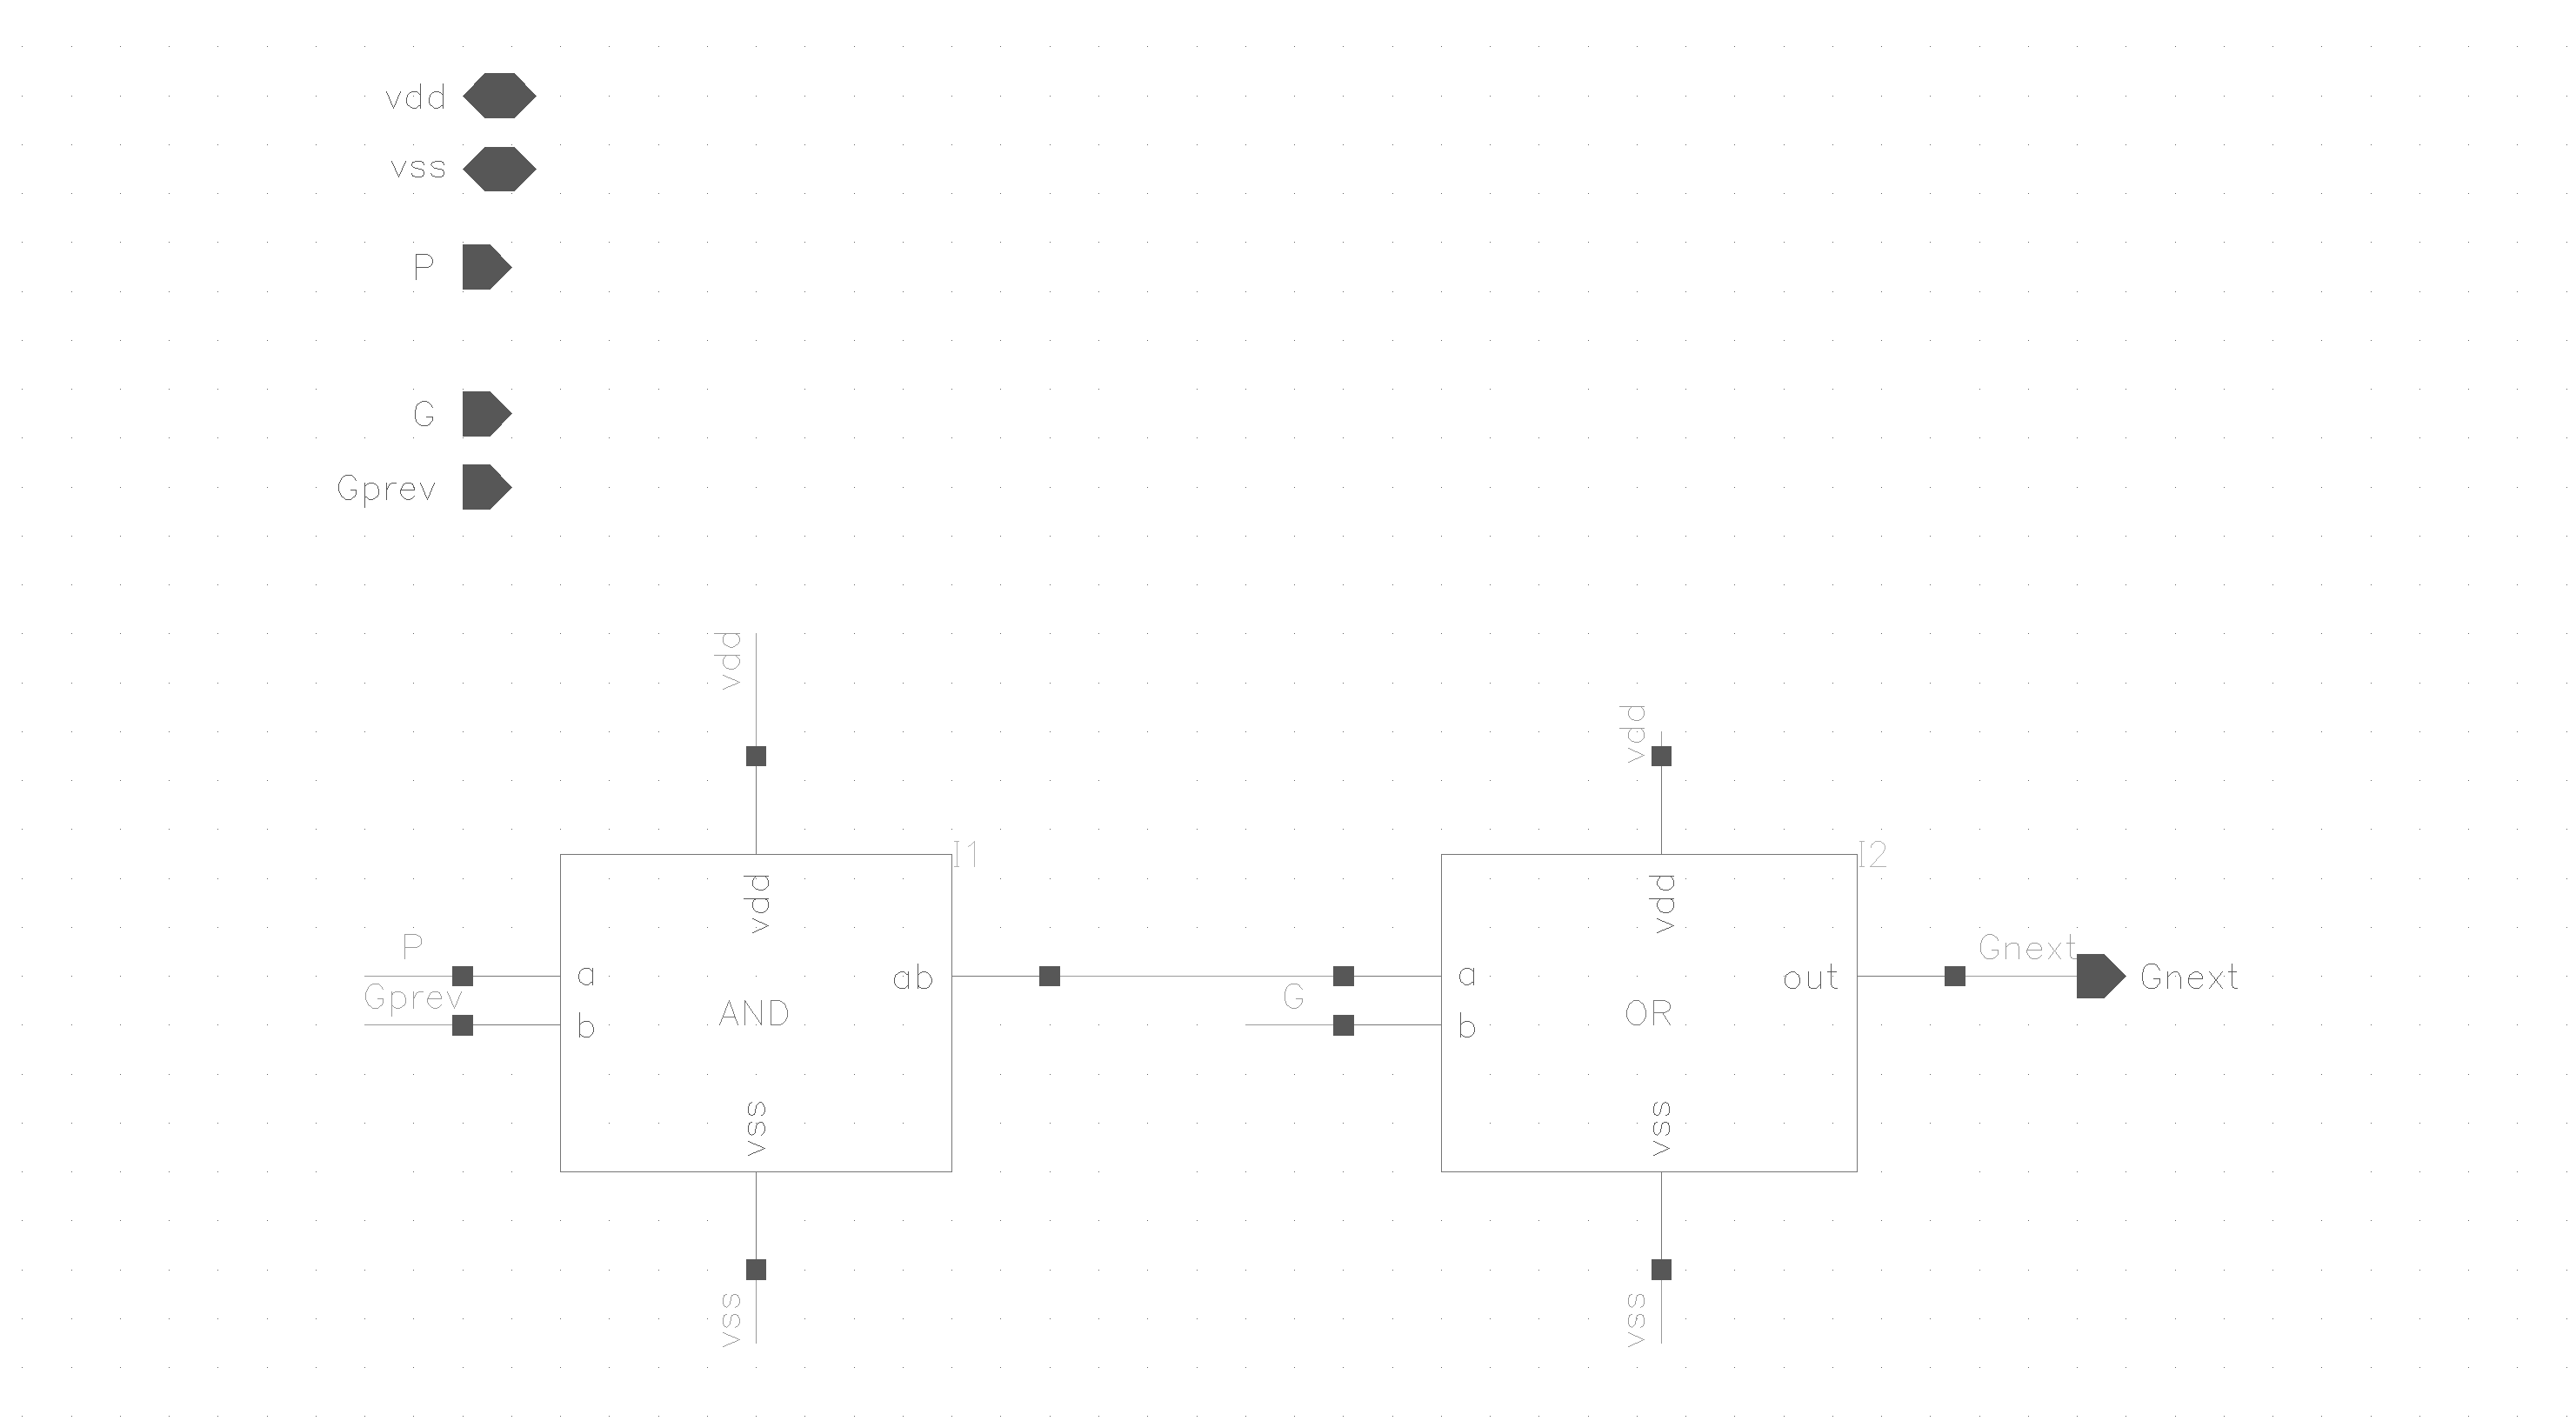
\includegraphics[width=1.2\textwidth]{../figures/yellow_carry}}
  \caption{Schematic view of the yellow carry block.} \label{fig:yellow_c}
\end{figure}

\begin{figure}[H]
  \centering
  \captionsetup{justification=centering}
  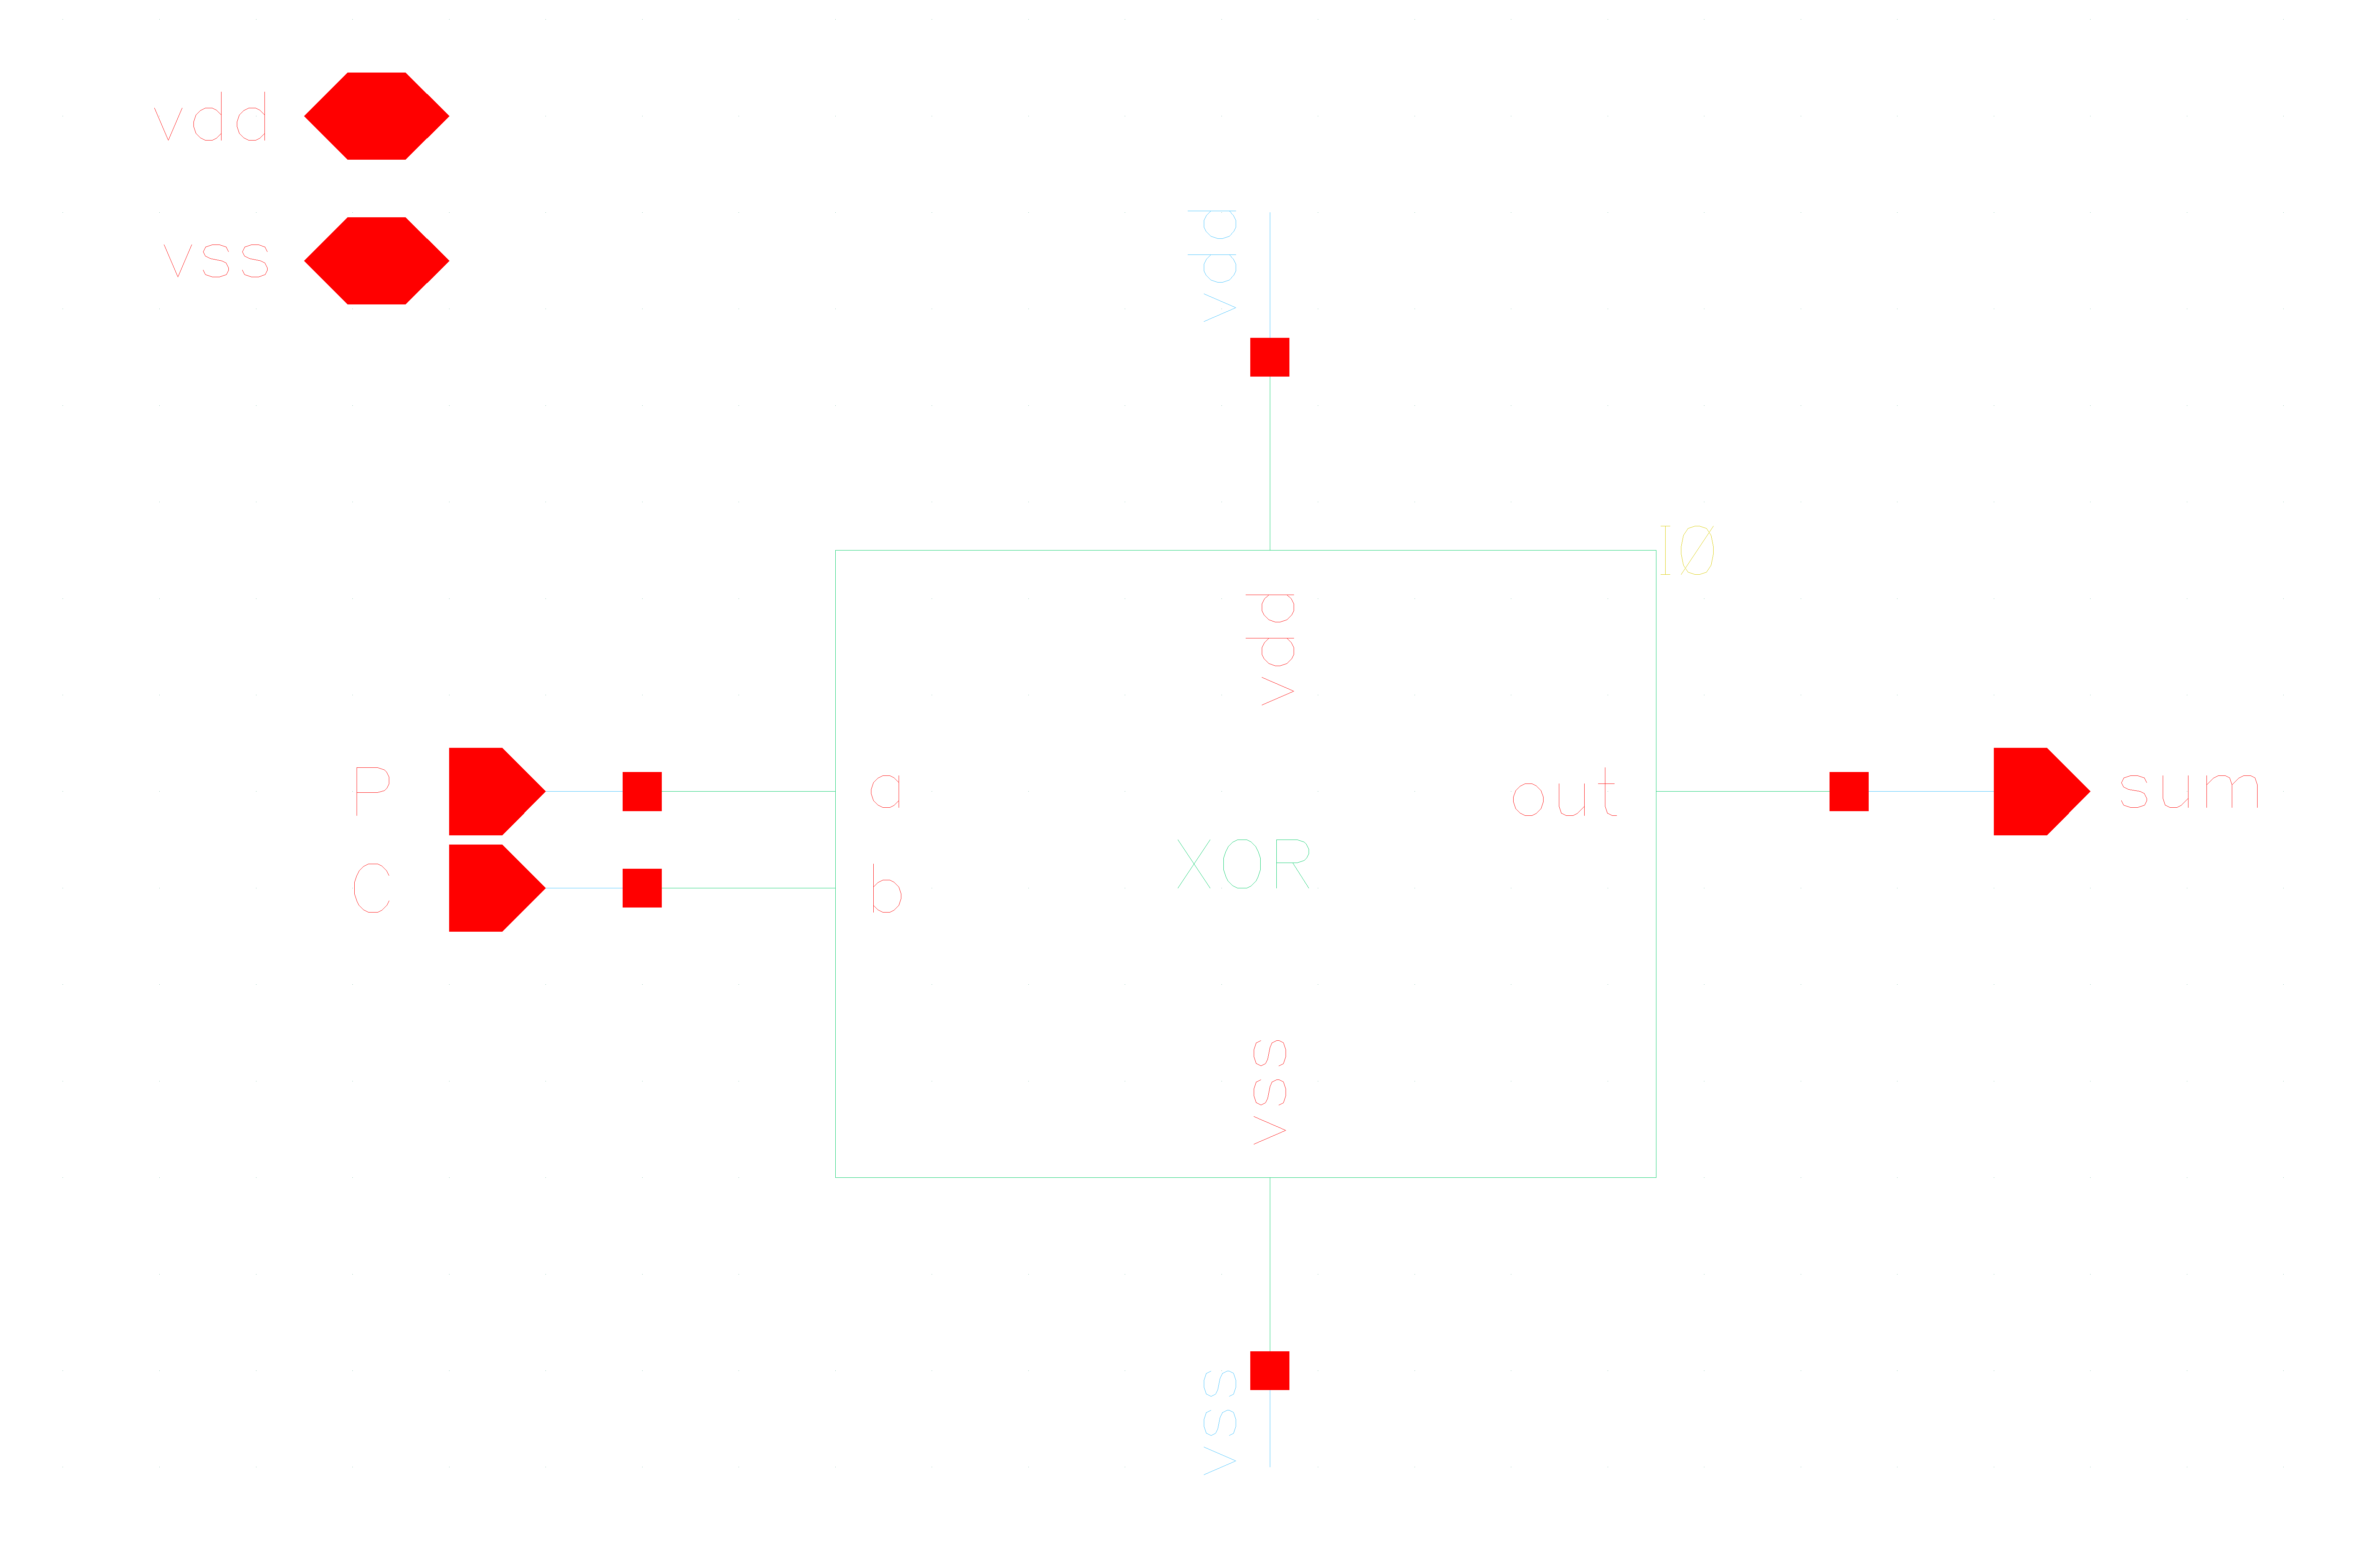
\includegraphics[clip,width=1.0\textwidth]{../figures/sum}
  \caption{Schematic view of the sum block.} \label{fig:sum}
\end{figure}

\subsection{Comparator}
The comparator consists of 17 2-input XNOR gates where one bit of each number is fed into each gate. The output from the XNOR gates are fed into a couple of AND gates which generates the final output. The comparator is 17 bits wide since it compares two 16 bit numbers plus their carry bits. The logic table of the XNOR gates is shown in table \ref{tab:xnor}.

\begin{table}[H]
  \caption{Logic table of XNOR block.}
  \centering
  \begin{tabular}{cc|c}
    \toprule
    $A_i$ & $B_i$ & $Y = \overline{(A_i \oplus B_i)}$ \\
    \midrule
    0 & 0 & 1 \\
    0 & 1 & 0 \\
    1 & 0 & 0 \\
    1 & 1 & 1 \\
    \bottomrule
    \label{tab:xnor}
  \end{tabular}
\end{table}


\section{Simulation Results} \label{sec:simulation_results}
%This section describes the high level simulation results. As simulations with too many signals were consuming too much memory (and crashed) the group decided to only look at signals that showed if the chip worked or not.\\


%\subsection{Adder}
%In Fig. \ref{adder_sim} simulation of the propagation delay through the adder %can be seen. Due to routing problems it was shown that bit 8 of the sum were %the slowest and as can be seen, it takes approximately 2.7ns from system clock %edge until the result is ready. \\

%\subsection{SPI output}
%In Fig. \ref{spi_out_sim} the four enable signals, the spi clock and the spi enale signal from the spi output module is shown. As can be seen, the four enable signals each goes high once during the high period of the spi enable.\\
%When the spi enable signal goes low the most significant bit of the sum is available on the first falling edge of the spi clock. If you look closely, you can see that the first sum outputted are the same as the first correction sum that can be seen in table \ref{tab:test_data}. (all sums match except for the third correction sum which contains an error)\\

%\subsection{BIST}
%In Fig. \ref{bist_sim} a simulation of the BISTout signal can be seen. As mentioned earlier the correction sum contains an error which makes the BISTout signal go low for one cycle. \\
%It can also be seen that the BISTout first go high after two system clock cycles as effect from pipelining.\\

After running the simulation for different corners we retrieved the following data regarding system performance. The test data used can be seen in Tab. \ref{tab:test_data}.

\begin{table}[H]
	\caption{Corner results.}
	\centering
	\begin{tabular}{| l | c | c | c | c |}
		\hline
		Corner & Nominal & Worst speed & Worst power & Unit\\
		\hline
		Simulated temperature & $27$ & $100$ & $0$ & Celcius\\
		\hline 
		Tested frequency & $200$ & $166$ & $333$ & MHz  \\
		\hline
		Power consumption chip & $18.89$ & $16.54$ & $31.3$ & mW \\
		\hline 
		Power consumption adder & $0.93$ & $0.807$ & $1.436$ & mW \\
		\hline 
		Propagation delay sum15 & $2.209$ & $4.234$ & $1.264$ & ns \\
		\hline 
		Propagation delay cout & $2.195$ & $3.744$ & $1.332$ & ns \\
		\hline
		Possible adder frequency & $455$ & $236$ & $750$ & MHz \\
		\hline
	\end{tabular}
	\label{corner_result}
\end{table}

The propagation delay was measured between Cin and Cout and between Cin and Sum15. The possible adder frequencies in Tab. \ref{corner_result} are based on longest of these two. One thing to note is that the complete system did not function correctly during worst speed. The adder itself works fine and the correct data is outputted through SPI-out, but the built-in self test is failing.

Simulation results, for the nominal corner with a frequency of 200 MHz, of the propagation delay, the SPI-out data and of BISTout can be seen in Appendix \ref{app:simulations}.


\section{Risks and Delays}


\begin{appendix}

\section{Time Plan}

\section{Time Report}

\end{appendix}

\end{document}
